\chapter{Massa e volume}\label{ch:g6:mass-and-volume}

Quanta limonada cabe na garrafa, e qual é o \omterm{def:g4:weight-and-mass:weight}{peso} do engradado de
garrafas? Duas perguntas diferentes --- espaço e material --- que a
conversa do dia a dia embaralha alegremente numa palavra só,
``grande''. A ciência desembaraça: \omterm{def:g6:mass-and-volume:volume}{volume} para o espaço que uma coisa
ocupa, \omterm{def:g3:measuring-mass:mass}{massa} para o material que ela contém. \omterm{def:g6:measurement-in-science:measuring}{Medir} a segunda você já
faz de olhos fechados; hoje aprendemos a \omterm{def:g6:measurement-in-science:measuring}{medir} a primeira --- até
para um seixo sem formato nenhum que uma régua pudesse amar.

\section{Volume: o espaço que uma coisa ocupa}

\begin{definition}[Volume]\label{def:g6:mass-and-volume:volume}
O \emph{volume}\index{volume} de uma coisa é a quantidade de espaço
que ela ocupa. \omterm{def:g3:solids-liquids-gases:solid}{Sólidos}, \omterm{def:g3:solids-liquids-gases:liquid}{líquidos} e gases têm volume: o tijolo ocupa o
espaço dele, a limonada ocupa o interior da garrafa, o \omterm{def:g2:air-around-us:air}{ar} ocupa o
resto. O volume é medido em \emph{centímetros
cúbicos}\index{centímetro cúbico} (\unit{cm^3}) --- o espaço de um
cubinho de um \omterm{def:g2:measuring-length:units}{centímetro} de aresta --- e em
\emph{litros}\index{litro} (\unit{L}).
\end{definition}

\begin{proposition}[O litro em cubinhos]\label{prop:g6:mass-and-volume:litre}
As duas famílias de \omterm{def:g6:measurement-in-science:measuring}{unidades} de \omterm{def:g6:mass-and-volume:volume}{volume} são uma só família:
\[
\qty{1}{L} = \qty{1000}{cm^3},
\qquad
\qty{1}{mL} = \qty{1}{cm^3}.
\]
Um \omterm{def:g6:mass-and-volume:volume}{litro} é exatamente o espaço dentro de um cubo de dez \omterm{def:g2:measuring-length:units}{centímetros}
de aresta: $10 \times 10 \times 10 = 1000$ cubinhos.
\end{proposition}

\begin{omfigure}
\begin{tikzpicture}[scale=0.85]
  \draw[thick] (0,0) rectangle (3,3);
  \draw[thick] (0,3) -- (0.9,3.75) -- (3.9,3.75) -- (3,3);
  \draw[thick] (3.9,3.75) -- (3.9,0.75) -- (3,0);
  \foreach \i in {1,...,9} {
    \draw[very thin] (0,0.3*\i) -- (3,0.3*\i);
    \draw[very thin] (0.3*\i,0) -- (0.3*\i,3);
    \draw[very thin] (0.3*\i,3) -- (0.3*\i+0.9,3.75);
    \draw[very thin] (3,0.3*\i) -- (3.9,0.3*\i+0.75);
    \draw[very thin] (0.09*\i,3+0.075*\i) -- (3+0.09*\i,3+0.075*\i);
    \draw[very thin] (3+0.09*\i,0.075*\i) -- (3+0.09*\i,3+0.075*\i);
  }
  \draw[thick, fill=omDef, fill opacity=0.6]
    (0,2.7) rectangle (0.3,3);
  \node[right, font=\small] at (4.6,3.0)
    {o cubo grande: \qty{10}{cm} de aresta};
  \node[right, font=\small] at (4.6,2.2)
    {$10 \times 10 \times 10 = 1000$ cubinhos};
  \node[right, font=\small] at (4.6,1.4)
    {cada cubinho: \qty{1}{cm^3}};
  \node[right, font=\small, omDef] at (4.6,0.6)
    {o todo: $\qty{1000}{cm^3} = \qty{1}{L}$};
\end{tikzpicture}

{\small Um \omterm{def:g6:mass-and-volume:volume}{litro}, desempacotado: mil cubinhos de um \omterm{def:g2:measuring-length:units}{centímetro}
empilhados dez por dez por dez.}
\end{omfigure}

\begin{example}[Volumes para saber de cor]\label{ex:g6:mass-and-volume:byheart}
Uma colher de chá leva cerca de \qty{5}{mL}; um copo de beber, cerca
de \qty{25}{cL}, um quarto de \omterm{def:g6:mass-and-volume:volume}{litro}; a caixa de leite, \qty{1}{L};
uma banheira, uns \qty{150}{L}; um cubinho de açúcar ocupa cerca de
\qty{3}{cm^3}; um dado, cerca de \qty{4}{cm^3}. Âncoras como essas
tornam possível o passo do julgamento em toda medida.
\end{example}

\section{Medir líquidos}

\begin{method}[Ler uma proveta]\label{met:g6:mass-and-volume:cylinder}
A jarra do laboratório é a \emph{proveta}: alta, estreita, com
graduação fina.
\begin{enumerate}
  \item ponha a proveta sobre uma mesa plana --- nunca faça a leitura
        com ela na mão;
  \item descubra o valor da graduação, como em toda escala;
  \item ponha o olho na mesma altura da superfície do \omterm{def:g3:solids-liquids-gases:liquid}{líquido}: a
        superfície não é plana, e sim levemente curva --- um
        \emph{menisco}\index{menisco} --- que sobe um pouquinho pelas
        paredes de vidro;
  \item faça a leitura no \emph{fundo} da curva, olhando bem de
        frente.
\end{enumerate}
Olho alto ou baixo demais, e a curva mente para você em um ou dois
passinhos --- o erro da vista de lado no disfarce predileto dele.
\end{method}

\begin{omfigure}
\begin{tikzpicture}[scale=0.85]
  \draw[thick] (1.0,0) -- (1.0,4.2) (3.0,0) -- (3.0,4.2);
  \draw[thick] (1.0,0) -- (3.0,0);
  \fill[omDef, opacity=0.2] (1.0,0.05) rectangle (3.0,2.6);
  \draw[omDef, very thick]
    (1.0,2.75) .. controls (1.6,2.55) and (2.4,2.55) .. (3.0,2.75);
  \foreach \y/\l in {0.6/10, 1.4/20, 2.2/30, 3.0/40, 3.8/50} {
    \draw (3.0,\y) -- (3.25,\y);
    \node[right, font=\footnotesize] at (3.3,\y) {\l};
  }
  \draw[-Stealth, omThm, thick] (6.3,2.6) -- (2.2,2.6);
  \node[right, font=\small, omThm] at (6.4,2.6)
    {leia no fundo da curva: \qty{28}{mL}};
  \node[below, font=\small] at (2.0,-0.35)
    {olho na altura da superfície, proveta sobre a mesa};
\end{tikzpicture}

{\small O \omterm{met:g6:mass-and-volume:cylinder}{menisco}: os \omterm{def:g3:solids-liquids-gases:liquid}{líquidos} sobem um pouquinho pelo vidro. A
leitura honesta é no fundo da curva, com o olho na altura dela.}
\end{omfigure}

\begin{omfigure}
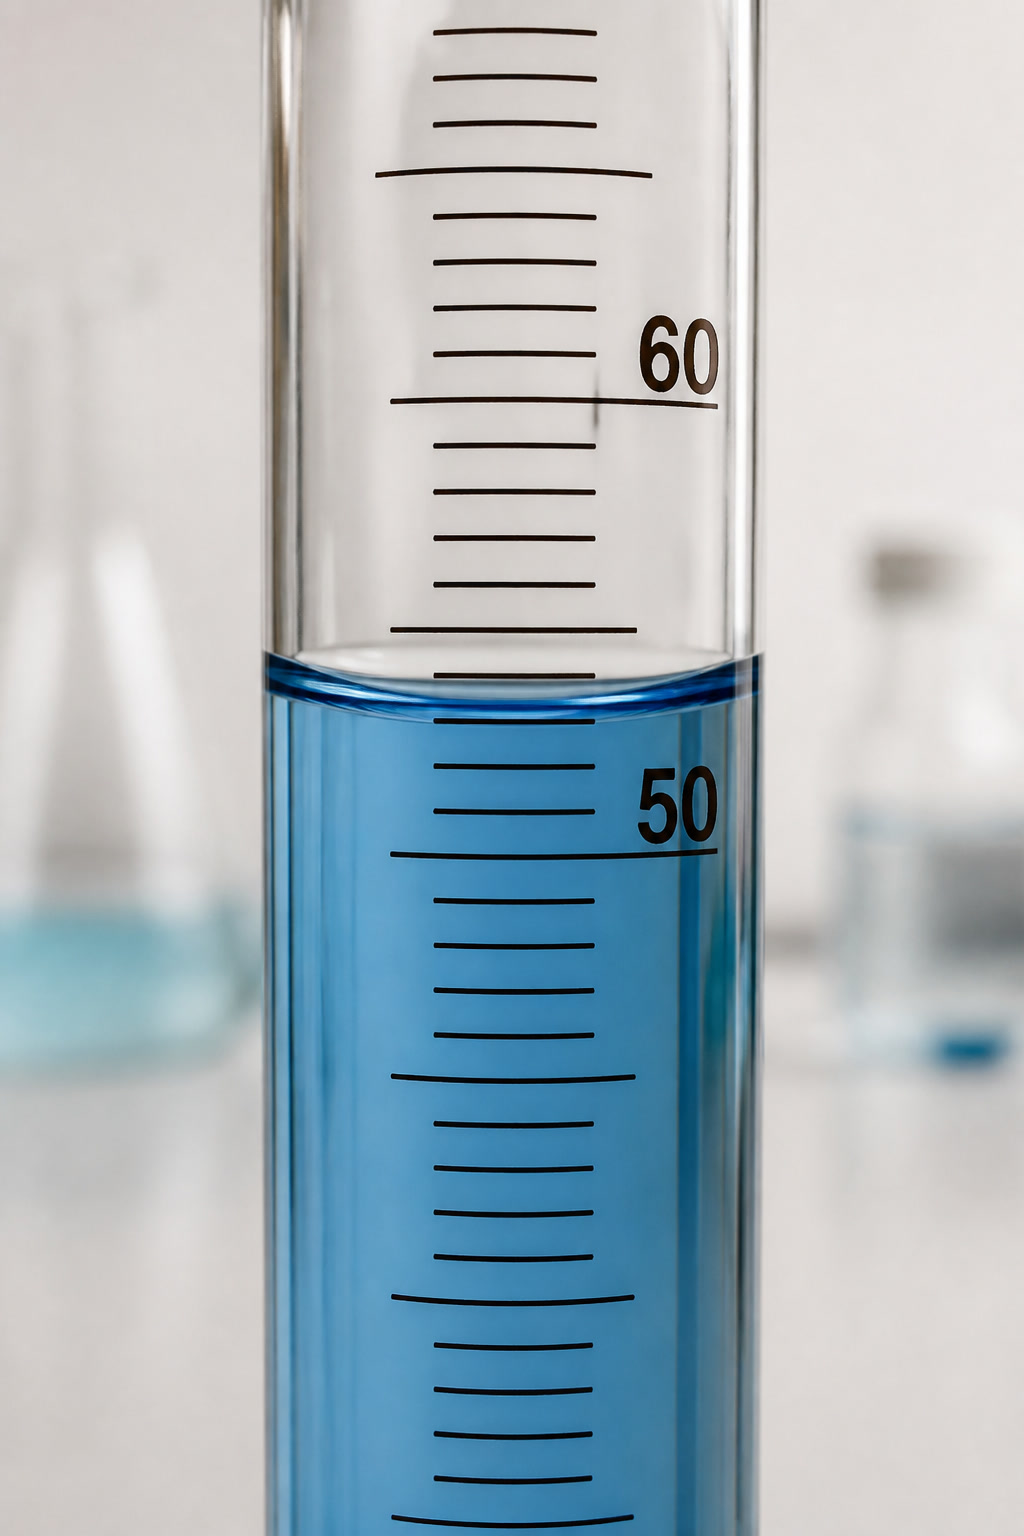
\includegraphics[width=0.3\linewidth]{images/book1/ai/g6-volume-cylinder.jpg}

{\small O \omterm{met:g6:mass-and-volume:cylinder}{menisco} de perto: leia o meio achatado da curva, com o olho na altura dele.}
\end{omfigure}

\section{Medir sólidos --- até os disformes}

Um \omterm{def:g3:solids-liquids-gases:solid}{sólido} em formato de tijolo se rende à régua: comprimento vezes
largura vezes altura dá o \omterm{def:g6:mass-and-volume:volume}{volume} dele em \unit{cm^3}, como o seu
curso de matemática mostrou. Mas e um seixo, uma chave, uma ameixa?
Régua nenhuma serve para um pedaço disforme. A resposta tem dois mil
anos, e saiu de uma banheira.

\begin{proposition}[Deslocamento]\label{prop:g6:mass-and-volume:displacement}
Um \omterm{def:g3:solids-liquids-gases:solid}{sólido} mergulhado completamente na água empurra para o lado ---
desloca --- exatamente o próprio \omterm{def:g6:mass-and-volume:volume}{volume} de água. A subida do nível da
água mede o intruso: disforme ou liso, a água se molda a cada
reentrância e a cada saliência.
\end{proposition}

\begin{method}[Volume pela subida da água]\label{met:g6:mass-and-volume:rise}
\begin{enumerate}
  \item despeje água numa proveta --- o bastante para cobrir o objeto
        --- e leia o \omterm{def:g6:mass-and-volume:volume}{volume}: digamos \qty{120}{mL};
  \item amarre uma linha no objeto e desça-o com cuidado até ele
        ficar todo debaixo d'água, sem respingo e sem encostar nas
        paredes;
  \item leia de novo: digamos \qty{145}{mL};
  \item subtraia: $145 - 120 = 25$ --- o \omterm{def:g6:mass-and-volume:volume}{volume} do objeto é
        \qty{25}{cm^3} (mililitros de subida, \omterm{def:g6:mass-and-volume:volume}{centímetros cúbicos} de
        pedra: a mesma coisa).
\end{enumerate}
\end{method}

\begin{omfigure}
\begin{tikzpicture}[scale=0.85]
  \draw[thick] (0.8,0) -- (0.8,3.6) (2.6,0) -- (2.6,3.6)
    (0.8,0) -- (2.6,0);
  \fill[omDef, opacity=0.2] (0.8,0.05) rectangle (2.6,2.0);
  \draw[omDef, very thick] (0.8,2.0) -- (2.6,2.0);
  \node[right, font=\footnotesize] at (2.7,2.0) {120};
  \node[below, font=\small] at (1.7,-0.3) {antes};
  \draw[thick] (6.2,0) -- (6.2,3.6) (8.0,0) -- (8.0,3.6)
    (6.2,0) -- (8.0,0);
  \fill[omDef, opacity=0.2] (6.2,0.05) rectangle (8.0,2.42);
  \draw[omDef, very thick] (6.2,2.42) -- (8.0,2.42);
  \node[right, font=\footnotesize] at (8.1,2.42) {145};
  \draw (7.1,3.6) -- (7.1,1.0);
  \fill[omExo] (7.1,0.75) ellipse (0.4 and 0.3);
  \node[below, font=\small] at (7.1,-0.3)
    {depois: o seixo, todo submerso};
  \draw[-Stealth, omThm, thick] (4.0,2.0) -- (5.6,2.35);
  \node[below, font=\small, omThm] at (4.8,1.9)
    {subida: \qty{25}{mL}};
\end{tikzpicture}

{\small O método da subida: a água sobe exatamente o \omterm{def:g6:mass-and-volume:volume}{volume} do seixo
--- $145 - 120 = \qty{25}{cm^3}$ de seixo.}
\end{omfigure}

\begin{example}[A coroa na banheira]\label{ex:g6:mass-and-volume:archimedes}
A velha história: um rei desconfiou que o ourives dele tinha
misturado prata ao ouro da coroa real e pediu ao cientista Arquimedes
que descobrisse a verdade sem danificar a coroa. Ao entrar numa
banheira cheia, Arquimedes viu a água transbordar pela borda --- e
percebeu num relâmpago que o transbordamento media o \omterm{def:g6:mass-and-volume:volume}{volume} do
próprio corpo dele, saliências e tudo. A lenda diz que ele saiu
correndo pelas ruas gritando ``Eureca!'' --- \emph{achei!} Como o
\omterm{def:g6:mass-and-volume:volume}{volume} da coroa desmascarou a fraude ainda precisa de mais uma ideia,
dois capítulos adiante; a banheira lhe deu o \omterm{def:g6:mass-and-volume:volume}{volume} de \emph{qualquer
coisa}.
\end{example}

\section{Massa e volume são respostas diferentes}

\begin{example}[Mesmo volume, massas diferentes]\label{ex:g6:mass-and-volume:different}
Encha dois copos iguais de \qty{25}{cL}, um com água e outro com mel,
e pese os dois (descontando os copos): o copo de mel guarda
nitidamente mais \omterm{def:g3:measuring-mass:units}{gramas} no mesmíssimo espaço. Mesmo \omterm{def:g6:mass-and-volume:volume}{volume}, \omterm{def:g3:measuring-mass:mass}{massas}
diferentes. E um \omterm{def:g6:mass-and-volume:volume}{litro} de \omterm{def:g2:air-around-us:air}{ar} pesa pouco mais que um \omterm{def:g3:measuring-mass:units}{grama}, no mesmo
espaço em que um \omterm{def:g6:mass-and-volume:volume}{litro} de água pesa um \omterm{def:g3:measuring-mass:units}{quilograma} inteiro. Espaço e
material são mesmo dois contadores diferentes --- segure firme essa
ideia: ela vira uma lei, com nome e tudo, no último capítulo deste
ano.
\end{example}

\begin{remark}[Pesar o que não fica em pé sozinho]\label{rem:g6:mass-and-volume:tare}
Como pesar farinha sem pesar a tigela dela? As balanças modernas têm
um botão para isso: ponha a tigela vazia no prato, aperte --- o
mostrador volta a zero --- e depois despeje: a balança agora informa
só a farinha. A manobra se chama \emph{tara}. Sem o botão, pese duas
vezes e subtraia: tigela-com-farinha menos tigela vazia. De um jeito
ou de outro, é de novo a regra do começo justo: partir de um zero
honesto.
\end{remark}

\section{Exercícios}

\begin{exercise}[$\star$]\label{exo:g6:mass-and-volume:1}
Que pergunta o \omterm{def:g6:mass-and-volume:volume}{volume} responde, e que pergunta a \omterm{def:g3:measuring-mass:mass}{massa} responde? Dê
as duas principais \omterm{def:g6:measurement-in-science:measuring}{unidades} de cada um.
\end{exercise}

\begin{exercise}[$\star$]\label{exo:g6:mass-and-volume:2}
Converta: \qty{2}{L} para \unit{cm^3}; \ \qty{350}{mL} para
\unit{cm^3}; \ \qty{1500}{cm^3} para \omterm{def:g6:mass-and-volume:volume}{litros}; \ meio \omterm{def:g6:mass-and-volume:volume}{litro} para
mililitros.
\end{exercise}

\begin{exercise}[$\star$]\label{exo:g6:mass-and-volume:3}
Por que uma proveta precisa ser lida na altura do olho, sobre a mesa
e no fundo do \omterm{met:g6:mass-and-volume:cylinder}{menisco}? Diga o erro que cada regra evita.
\end{exercise}

\begin{exercise}[$\star$]\label{exo:g6:mass-and-volume:4}
Uma proveta marca \qty{200}{mL}; com uma ameixa mergulhada, ela marca
\qty{265}{mL}. Qual é o \omterm{def:g6:mass-and-volume:volume}{volume} da ameixa, em \unit{cm^3}?
\end{exercise}

\begin{exercise}[$\star$]\label{exo:g6:mass-and-volume:5}
Por que o método da subida funciona até para um seixo disforme, se
régua nenhuma conseguiria medi-lo? Qual proposição responde?
\end{exercise}

\begin{exercise}[$\star$]\label{exo:g6:mass-and-volume:6}
Uma borracha em formato de tijolinho mede \qty{5}{cm} por \qty{2}{cm}
por \qty{1}{cm}. Qual é o \omterm{def:g6:mass-and-volume:volume}{volume} dela? Plano de conferência: como
você confirmaria isso com o método da subida?
\end{exercise}

\begin{exercise}[$\star$]\label{exo:g6:mass-and-volume:7}
Para pesar arroz: tigela vazia \qty{280}{g}; tigela com arroz
\qty{745}{g}. Quanto arroz há? Qual botão faz o mesmo serviço num
passo só?
\end{exercise}

\begin{exercise}[$\star$]\label{exo:g6:mass-and-volume:8}
Qual tem o maior \omterm{def:g6:mass-and-volume:volume}{volume}, um \omterm{def:g3:measuring-mass:units}{quilograma} de penas ou um \omterm{def:g3:measuring-mass:units}{quilograma} de
ferro? Qual tem a maior \omterm{def:g3:measuring-mass:mass}{massa}? (Responda os dois com cuidado.)
\end{exercise}

\begin{exercise}[$\star\star$]\label{exo:g6:mass-and-volume:9}
O método da subida falha para uma rolha: ela \omterm{def:g1:floating-and-sinking:words}{flutua}. Proponha uma
solução que ainda use a proveta --- e diga o que precisa ser
subtraído se a sua solução usar um objeto ajudante.
\end{exercise}

\begin{exercise}[$\star\star$]\label{exo:g6:mass-and-volume:10}
Uma caixa de suco diz conter \qty{1}{L}. Despejada, ela enche três
vezes um copo de \qty{250}{mL} e o quarto copo só até a marca de
\qty{200}{mL}. A declaração era honesta? Por quanto?
\end{exercise}

\begin{exercise}[$\star\star$]\label{exo:g6:mass-and-volume:11}
Um colar é mergulhado numa proveta que marcava \qty{80.0}{mL}; ela
sobe para \qty{83.5}{mL}. O joalheiro afirma que o colar contém
\qty{5}{cm^3} de ouro. A afirmação pode ser verdadeira? O que,
exatamente, a água mediu?
\end{exercise}

\begin{exercise}[$\star\star\star$]\label{exo:g6:mass-and-volume:12}
Projete uma conferência estilo banheira da própria
\cref{prop:g6:mass-and-volume:displacement}, usando um objeto em
formato de tijolo cujo \omterm{def:g6:mass-and-volume:volume}{volume} a régua já conhece. Descreva os passos,
preveja as duas leituras da proveta para um bloco de
$4 \times 3 \times 2$ \omterm{def:g2:measuring-length:units}{centímetros} mergulhado em \qty{150}{mL} e diga
que resultado provaria que a proposição está errada.
\end{exercise}

\section{Problema: Dia de engarrafamento no pomar}

\begin{problem}[{Problema de fim de semana --- dia de prensa no
pomar; litros virando garrafas, engradados subindo na balança; o
seixo na jarra}]\label{pb:g6:mass-and-volume:1}
O pomar prensa as maçãs hoje, e cada ajudante ganha um serviço de
medição.

\medskip\noindent\textbf{Parte I --- Suco por \omterm{def:g6:mass-and-volume:volume}{litro}.}
A prensa encheu um barril de \qty{20}{L}.
\begin{enumerate}
  \item Quantos \omterm{def:g6:mass-and-volume:volume}{centímetros cúbicos} são \qty{20}{L}?
  \item O suco é engarrafado em garrafas de \qty{75}{cL}. Quantas
        garrafas \emph{cheias} o barril dá?
  \item Quanto suco sobra depois da última garrafa cheia, em
        centilitros?
  \item A sobra é despejada em copos de \qty{25}{cL}. Quantos copos
        ela enche?
\end{enumerate}

\medskip\noindent\textbf{Parte II --- Engradados na balança.}
\begin{enumerate}[resume]
  \item Uma garrafa vazia tem \omterm{def:g3:measuring-mass:mass}{massa} de \qty{450}{g}. Usando a Parte
        I, qual é a \omterm{def:g3:measuring-mass:mass}{massa} do suco de uma garrafa cheia, se um \omterm{def:g6:mass-and-volume:volume}{litro}
        de suco tem \omterm{def:g3:measuring-mass:mass}{massa} de cerca de \qty{1}{kg}? (Trabalhe em
        \omterm{def:g3:measuring-mass:units}{gramas}.)
  \item Então quanto pesa uma garrafa cheia, ao todo?
  \item Um engradado de madeira pesa \qty{2}{kg} vazio e carrega seis
        garrafas cheias. Qual é a \omterm{def:g3:measuring-mass:mass}{massa} total de um engradado
        carregado?
  \item A perua pode levar \qty{200}{kg} de engradados. Quantos
        engradados carregados ela pode levar? (Só engradados
        inteiros.)
\end{enumerate}

\medskip\noindent\textbf{Parte III --- O seixo na jarra.}
O pequeno Tom deixa cair um seixo numa jarra cheia de \qty{1}{L} de
suco, e o suco transborda sobre a mesa.

\begin{enumerate}[resume]
  \item O suco transbordado, recolhido, mede \qty{40}{mL}. O que o
        derramamento mediu a respeito do seixo, e por qual
        proposição?
  \item Depois que o seixo é pescado de volta, quanto suco resta na
        jarra?
  \item Tom protesta: ``O seixo é pequeno --- olha, ele se esconde no
        meu punho!'' A irmã dele responde com uma proveta: ela põe o
        seixo em \qty{100}{mL} de água. Qual leitura prova que o
        derramamento disse a verdade?
  \item Contabilidade extra: o seixo pesa \qty{104}{g} na balança de
        cozinha. Sem nenhuma ideia nova, você já consegue dizer se o
        material do seixo é mais pesado ou mais leve que o material
        do suco \emph{para o mesmo espaço ocupado}? Compare
        \qty{104}{g} de seixo em \qty{40}{cm^3} com a \omterm{def:g3:measuring-mass:mass}{massa} de suco
        que encheria esses mesmos \qty{40}{cm^3} --- e guarde a sua
        conclusão quentinha para o capítulo da densidade.
\end{enumerate}
\end{problem}
